\documentclass[12pt]{report}
\usepackage[utf8]{inputenc}
\usepackage[a4paper, margin=1in]{geometry}
\usepackage{graphicx}
\usepackage{float}
\usepackage{titlesec}
\usepackage{setspace}
\usepackage{hyperref}

\title{\textbf{ParkX - Smart Parking Management System}\\ \Large Technical Documentation & Architectural Diagrams}
\author{Amal Biju}
\date{\today}

\begin{document}

\maketitle

\chapter*{Technical Overview}
This document provides a comprehensive visual breakdown of the ParkX Smart Parking Management System. The diagrams cover system actors, logical flows, architectural layering, data structures, and the engineering pipeline, strictly adhering to the project's Laravel 12 and PostgreSQL technical stack.

\newpage

\section*{Figure 1: UML Use Case Diagram}
The Use Case Diagram illustrates the interactions between the primary actors (Driver, Property Owner, and Super Admin) and the ParkX System boundary, detailing core functionalities like booking, venue management, and global governance.
\begin{figure}[H]
    \centering
    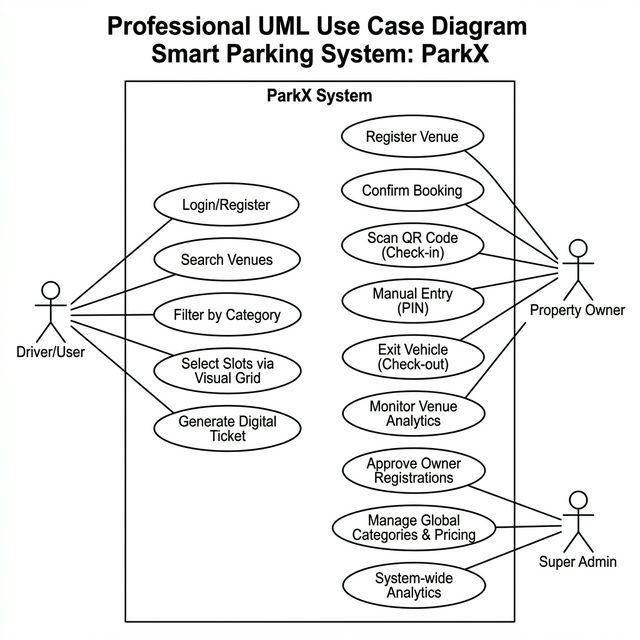
\includegraphics[width=0.9\textwidth]{diag_use_case.png}
    \caption{UML Use Case Diagram - System Boundary & Actors}
\end{figure}

\newpage

\section*{Figure 2: User Booking Activity Flow}
This activity diagram maps the logical decision points for a Driver, from initial venue search to the generation of a digital ticket with a 6-digit PIN.
\begin{figure}[H]
    \centering
    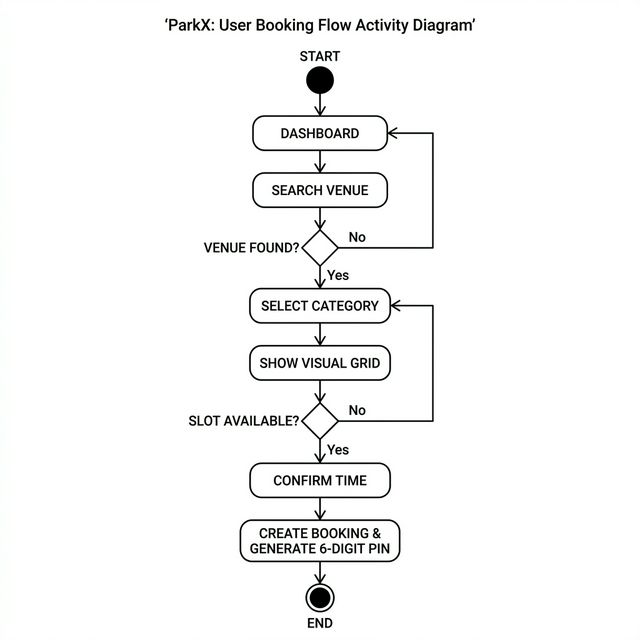
\includegraphics[width=0.9\textwidth]{diag_activity_booking.png}
    \caption{Activity Diagram - Reservation Logic}
\end{figure}

\newpage

\section*{Figure 3: Architectural Map Grid}
A direct mapping between Frontend UI components and their corresponding Laravel Backend Controllers, ensuring a clear understanding of the MVC implementation.
\begin{figure}[H]
    \centering
    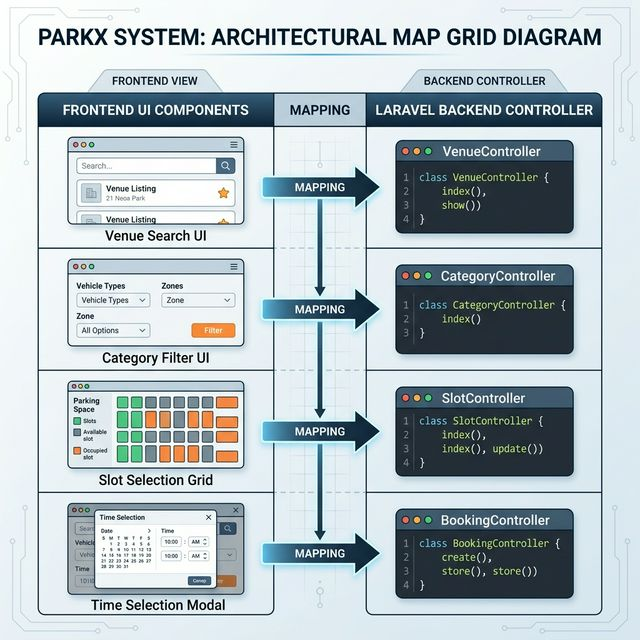
\includegraphics[width=0.9\textwidth]{diag_architectural_map.png}
    \caption{Logic/View Mapping Grid}
\end{figure}

\newpage

\section*{Figure 4: N-Tier System Architecture}
The system's structural layers, showing the separation between the Client Tier, Web Server (Apache), Application Tier (Laravel), and Data Tier (PostgreSQL).
\begin{figure}[H]
    \centering
    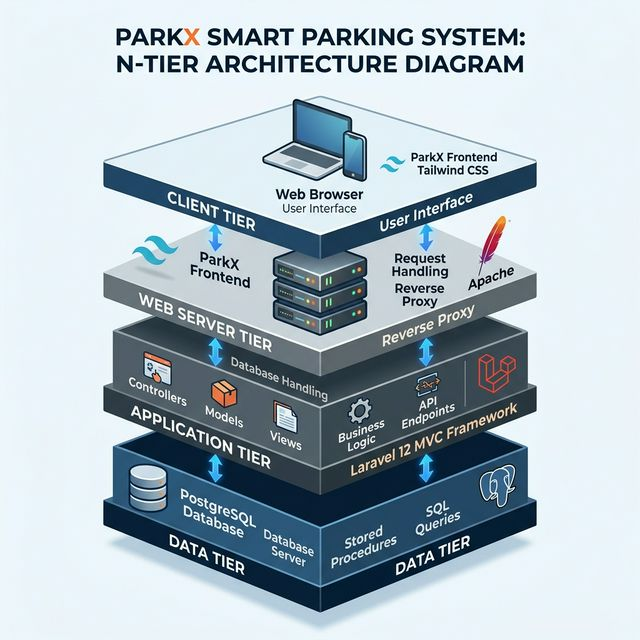
\includegraphics[width=0.9\textwidth]{diag_system_architecture.png}
    \caption{N-Tier Stack Visualization}
\end{figure}

\newpage

\section*{Figure 5: Class Diagram (Eloquent Models)}
Detailed UML Class Diagram showing the Laravel Eloquent models, their attributes, and multiplicities (1:M relationships).
\begin{figure}[H]
    \centering
    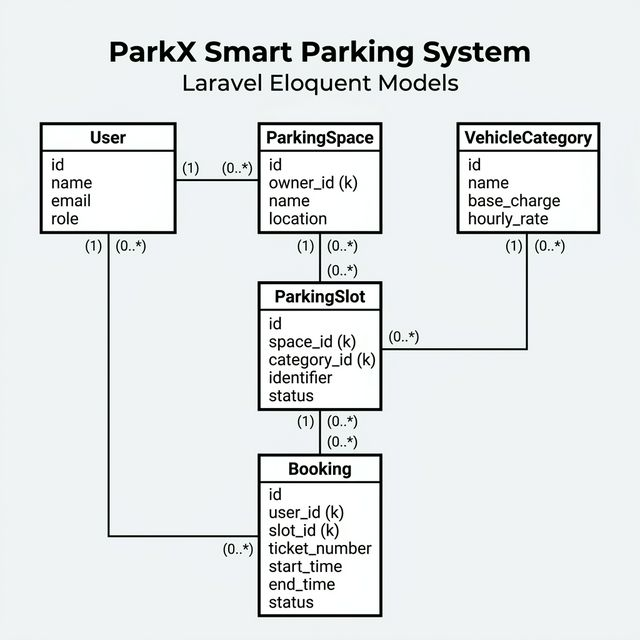
\includegraphics[width=0.9\textwidth]{diag_class_diagram_models.png}
    \caption{UML Class Diagram - Data Models}
\end{figure}

\newpage

\section*{Figure 6: Entity-Relationship (ER) Diagram}
Database schema visualization using Crow's Foot notation, detailing the PostgreSQL table structures, primary keys, and foreign key constraints.
\begin{figure}[H]
    \centering
    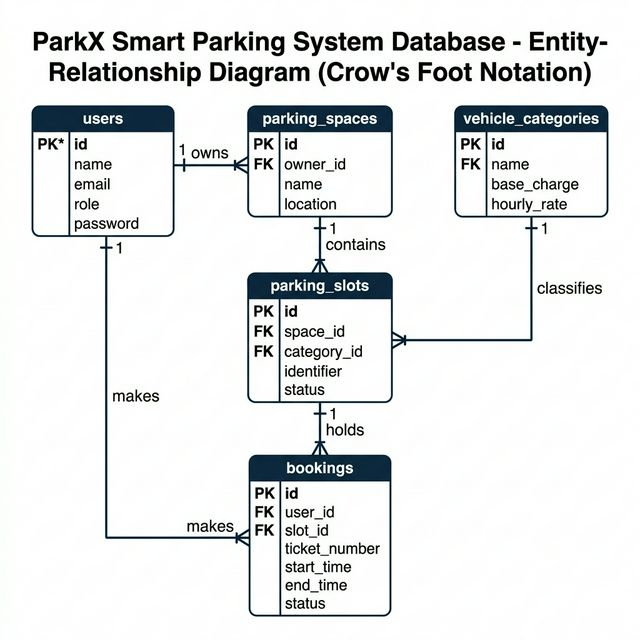
\includegraphics[width=0.9\textwidth]{diag_er_diagram_schema.png}
    \caption{PostgreSQL ER Diagram (Crow's Foot Notation)}
\end{figure}

\newpage

\section*{Figure 7: Transactional Locking Sequence}
A sequence diagram detailing the `SELECT ... FOR UPDATE` mechanism used during slot reservation to prevent race conditions and ensure data integrity.
\begin{figure}[H]
    \centering
    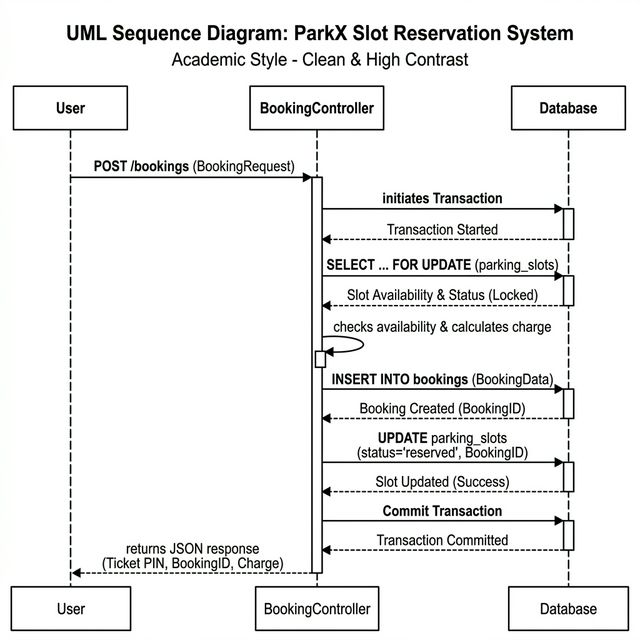
\includegraphics[width=0.9\textwidth]{diag_sequence_locking.png}
    \caption{Database Sequence Diagram - Transactional Logic}
\end{figure}

\newpage

\section*{Figure 8: Project Engineering Pipeline}
The end-to-end development lifecycle for ParkX, from local environment setup (XAMPP/VS Code) to production-ready deployment.
\begin{figure}[H]
    \centering
    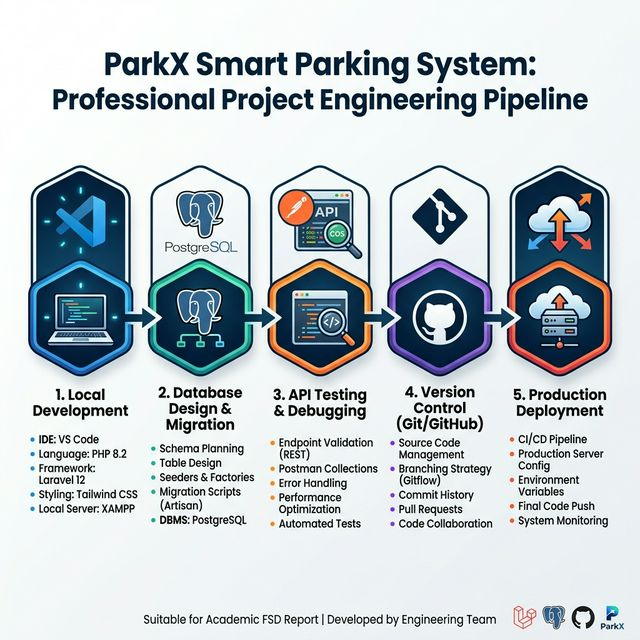
\includegraphics[width=0.9\textwidth]{diag_project_pipeline.png}
    \caption{Development & Deployment Pipeline}
\end{figure}

\end{document}
